\documentclass[conference]{IEEEtran}
\IEEEoverridecommandlockouts
\usepackage{cite}
\usepackage{amsmath,amssymb,amsfonts,amsthm}
\usepackage{graphicx}
\usepackage{booktabs}
\usepackage{xcolor}
\usepackage[hidelinks]{hyperref}

% ReS AI @ IROS 2026 workshop submission (4+N format, double-blind).
% Non-archival; content is a subset of the full conference submission.
\newcommand{\todo}[1]{\textcolor{red}{[TODO: #1]}}
\providecommand{\coloneqq}{\mathrel{:=}}

\title{\LARGE \bf The VLM Grounds Predicates, the Logic Decides:\\
Neuro-Symbolic Hazard Identification for Safe Steering\\of Frozen Vision-Language-Action Policies}

% Double-blind: no author block content.
\author{Anonymous submission to the IROS 2026 Workshop on Embodied\\
Neuro-Symbolic AI for Reliable and Safe Robotics (ReS AI)}

\graphicspath{{figs/}}

\begin{document}
\maketitle

\begin{abstract}
Runtime safety filters for vision-language-action (VLA) policies must first decide \emph{what} to avoid before any barrier can enforce \emph{how} to avoid it. We show that this identification problem has a sharply neuro-symbolic answer: a fixed three-literal first-order rule over VLM-groundable predicates,
$\textsc{Hazard}(x) \coloneqq \textsc{Protected}(x)\vee\textsc{Moving}(x)\vee(\lnot\textsc{Mentioned}(x)\wedge\textsc{NearestToPath}(x))$,
is statistically indistinguishable from ground-truth hazard identity in paired robot rollouts (all $p\ge0.18$), while every way of granting the VLM \emph{more} authority fails, and fails unsafe. Whole-scene VLM identification scores 18--64\% where the decomposed rule scores 100\%; runtime VLM \emph{composition} of the rule itself produces over-restrictive conjunctions that guard nothing --- the true hazard goes unguarded. The VLM's reliable role is answering local per-object predicates (\textsc{Referenced}, \textsc{Protected}): swapping hand-coded heuristics for VLM predicate grounding changes \emph{no} decision on 59 benchmark scenes while adding paraphrase competence no string heuristic has (``deliver it to me'' $\Rightarrow$ the hand is protected). The symbolic decision then drives a training-free steering layer inside the frozen $\pi_{0.5}$ flow policy's denoising, certified by a discrete control-barrier chain re-checked on executed actions. On the LIBERO-Safety benchmark the stack beats two dedicated safety-shield architectures by $+15$--$20$ task-success points at equal-or-lower violations, runs its fully perception-grounded tier at a quarter of the unshielded baseline's violation rate while beating it outright on the human-safety suite, and refuses unsafe instructions at 100/100/80\% versus the best published 80/72/36\% --- evidence that reliable embodied safety today is a \emph{division of labor}: neural components ground symbols and generate actions; a small, inspectable logic makes the safety-critical decisions.
\end{abstract}

\section{Introduction}
\label{sec:intro}

Vision-language-action (VLA) policies such as $\pi_{0.5}$~\cite{pi05} imitate expert demonstrations superbly and unsafely: on safety-augmented LIBERO benchmarks the frozen policy collides with a hazardous distractor in up to 86--88\% of episodes, and drives its gripper into a human hand in 40\% of episodes on the hardest suite of LIBERO-Safety~\cite{liberosafety}. A growing line of work responds with runtime enforcement --- control-barrier-function (CBF) shields and in-denoising guidance~\cite{sota2607,aegis,safediffuser} --- but every such mechanism presupposes an answer to a prior question: \emph{which} scene entity is the hazard, and \emph{what kind} of hazard is it?

This identification question is where the neuro-symbolic design space is widest, and where, we argue, the field's default instinct --- ask a large VLM to look at the scene and decide --- is measurably wrong. This paper contributes a controlled study of \emph{how much authority to give the neural component} in an embodied safety stack, with three findings:

\textbf{(1) A three-literal symbolic rule suffices.} A fixed first-order rule over four predicates (Sec.~\ref{sec:ident}) matches privileged ground-truth hazard identity in paired rollouts on a physical-safety benchmark: no significant difference on any success or collision axis (all $p\ge0.18$), with every trend favoring the rule. Ground-truth-free identification carries no measurable cost.

\textbf{(2) The VLM belongs at the predicate level.} Replacing the rule's hand-coded literal groundings with VLM-answered per-object predicates reproduces the identical decision on all 59 scenes of two benchmarks --- and resolves references no string heuristic can (``deliver it to me''). The neural component adds open-vocabulary competence exactly when its outputs are \emph{local, checkable, and composed by logic}.

\textbf{(3) More VLM authority fails unsafe.} Both natural escalations --- whole-scene VLM identification, and VLM \emph{composition} of the rule from a predicate library --- were implemented, pre-registered, and killed by their own gates (Sec.~\ref{sec:negative}). The characteristic composition failure is an over-restrictive conjunction that fires on nothing, leaving the true hazard unguarded: the system fails \emph{unsafe}, the worst direction for a safety component.

The symbolic decision layer feeds a training-free enforcement layer (Sec.~\ref{sec:enforce}) that steers the frozen policy's flow-matching denoising and re-verifies a discrete-CBF chain on the executed action prefix --- so the certificate is independent of which mechanism produced the action. We summarize system-level results on LIBERO-Safety (Sec.~\ref{sec:results}): violations of a never-safety-trained checkpoint eliminated on the physical suites, and the benchmark's safety-reasoning track swept by the symbolic instruction judge (100/100/80\% refusal vs.\ best published 80/72/36\%).

\begin{figure*}[t]
\centering
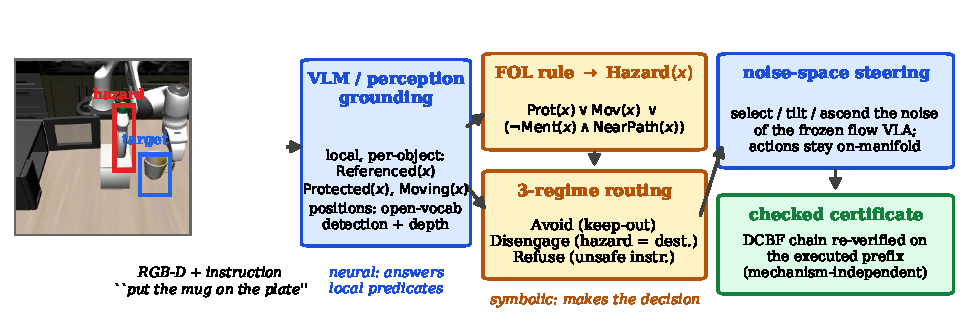
\includegraphics[width=0.98\textwidth]{fig_pipeline.pdf}
\caption{\textbf{The division of labor.} A real LIBERO-Safety scene (left; obstacle-avoidance suite) is processed by \emph{neural} components (blue) that only answer local, checkable questions --- per-object predicates and open-vocabulary localization --- while a fixed \emph{symbolic} layer (amber) makes every safety-critical decision: hazard election by the three-literal rule of Eq.~\eqref{eq:fol} and routing into avoid / disengage / refuse regimes. Enforcement searches the frozen flow policy's noise space over $K{=}8$ candidate chunks, and a discrete-CBF chain re-checked on the executed prefix (green) certifies the output independently of which neural search produced it; the certified 5-step prefix executes and the loop replans from the next observation.}
\label{fig:pipeline}
\end{figure*}

\section{Related Work}
\label{sec:related}

\textbf{Semantic safety constraints from VLMs.} Brunke et al.~\cite{brunke2025semantic} compile semantic constraints into motion safeguards via multi-prompt VLM querying; their corridor-exemption insight transfers to our setting. In-denoising CBF guidance for flow VLAs~\cite{sota2607} and diffusion-time barriers~\cite{safediffuser,cbf2602} address enforcement, assuming hazard identity given (typically from the simulator). Attention-reading approaches~\cite{yourmodel} extract identity from VLA internals. Our study isolates the identification layer and varies only the neural/symbolic division of labor.

\textbf{Neuro-symbolic robot safety.} The classical argument for symbolic layers --- inspectability, compositionality, verifiable failure modes --- meets a practical obstacle in open-world robotics: grounding. Our finding is an empirical resolution: grounding is exactly the subproblem modern VLMs solve reliably (local, per-object, verifiable predicates), while scene-level judgment and rule synthesis are exactly where they fail. This division echoes formal-methods-plus-perception architectures, but is here validated by paired ablations on physical safety benchmarks rather than by construction.

\section{Method}
\label{sec:method}

\subsection{Identification: a first-order rule over grounded predicates}
\label{sec:ident}

The scene-level decision of what to guard is made by a fixed three-literal rule:
\begin{equation}
\begin{aligned}
\textsc{Hazard}(x) \coloneqq{}& \textsc{Protected}(x)\ \vee\ \textsc{Moving}(x)\ \vee \\
&\big(\lnot\textsc{Mentioned}(x)\wedge\textsc{NearestToPath}(x)\big),
\end{aligned}
\label{eq:fol}
\end{equation}
ranked protected-first, then by path distance. \textsc{Protected} covers a semantic class (body parts, objects attached to a person) that is never mention-excluded; \textsc{Moving} is grounded online by settle-window displacement ($>$1\,cm), re-read at every replan --- this single class literal is what handles dynamic human-hand intruders. \textsc{Mentioned} performs reference resolution against the instruction; \textsc{NearestToPath} measures distance to the sanctioned reach segments (end-effector $\to$ target $\to$ destination).

\emph{Property-gated variant (affordance-class hazards).} Suites whose hazards are defined by object \emph{properties} rather than placement use a property theory with the same protected/moving core:
\begin{equation}
\begin{aligned}
\textsc{Hazard}(x) \coloneqq{}& \textsc{Protected}(x)\vee\textsc{Moving}(x)\ \vee\\
&\big(\textsc{Prop}(x)\wedge\lnot\textsc{Mentioned}(x)\wedge\lnot\textsc{Target}(x)\big),\\
\textsc{Prop}(x) \coloneqq{}& \textsc{Sharp}(x)\vee\textsc{Fragile}(x)\vee\textsc{HeatSrc}(x)\ \vee\\
&\big(\textsc{Hot}(x)\wedge\exists s{:}\,\textsc{HeatSrc}(s)\wedge d(x,s){<}0.15\big),
\end{aligned}
\label{eq:folprop}
\end{equation}
with \emph{no} near-path fallback: a scene with no property-positive object elects nothing (a correct no-op). The heat conjunct is genuinely first-order --- a hot object is hazardous only \emph{near an active heat source}, a two-entity, state-dependent condition no flat scorer expresses.

\emph{Two interchangeable grounding backends.} The literals can be grounded by (a) hand heuristics plus one-shot cached VLM hazard-property priors with a fail-safe floor (semantics may raise concern, never delete protection), or (b) \emph{VLM predicate grounding}: a small VLM (majority of 5 votes, cached per object class, runtime API-free) answers only local per-object questions --- \textsc{Referenced}$(x)$, \textsc{Protected}$(x)$, and the property literals of Eq.~\eqref{eq:folprop}. The rule, the ranking, and the routing below are identical under both backends; Table~\ref{tab:grounding} summarizes every literal's grounding. At evaluation time the entire symbolic stack runs API-free.

\begin{table}[t]
\centering
\caption{Every predicate and its grounding. ``VLM (cached)'' = one-shot offline majority-voted queries, zero runtime calls.}
\label{tab:grounding}
\small
\setlength{\tabcolsep}{4pt}
\begin{tabular}{ll}
\toprule
Predicate & Grounding \\
\midrule
\textsc{Protected}$(x)$ & semantic class (body parts, person-attached); \\
 & VLM-answerable variant identical on 59/59 scenes \\
\textsc{Moving}$(x)$ & online geometry: settle-window displ.\ $>$1\,cm, \\
 & re-read every replan \\
\textsc{Mentioned}$(x)$ & head-noun match vs.\ instruction \\
\textsc{NearestToPath}$(x)$ & distance to eef$\to$target$\to$dest segments \\
\textsc{Target}/dest & instruction / goal parse \\
\textsc{Hot/Sharp/Fragile/} & hand token lists (ablation) \emph{or} \\
\quad\textsc{HeatSrc}$(x)$ & VLM (cached) per object class \\
\textsc{Referenced}$(x)$ & reference resolution incl.\ paraphrase (VLM) \\
positions $\mathrm{pos}(x)$ & privileged sim (GT tier) or open-vocab \\
 & detection + depth (perception tier) \\
\bottomrule
\end{tabular}
\end{table}

\emph{Perception tier.} At the ground-truth-free tier, positions and extents come from open-vocabulary detection~\cite{gdino} back-projected through depth (median localization error 0.036--0.067\,m across benchmarks); collision \emph{scoring} remains simulator-anchored in all conditions.

\subsection{Three-regime routing}
\label{sec:routing}

Not every hazard is a keep-out; the symbolic layer routes each episode:
(1)~\textbf{Avoid} --- a geometric hazard off the task path: barrier-guided steering (Sec.~\ref{sec:enforce}).
(2)~\textbf{Duality disengage} --- the hazard \emph{is} the destination ($\textsc{Protected}(x)\wedge\textsc{Referenced}(x)$, or guard--destination overlap): geometric keep-out disengages; safety comes from routing. This regime is forced by human-handover suites, where the trained behavior already avoids hand contact and any keep-out only destroys the task.
(3)~\textbf{Refuse} --- the \emph{instruction itself} is the hazard: a rule-based semantic judge over (verb, patient, hazard-property) triples refuses execution before any motion.

Each regime is a symbolic, inspectable decision: the system can state \emph{which} literal fired and \emph{why} an episode was routed --- the interpretability property that motivates neuro-symbolic safety architectures in the first place.

\subsection{Enforcement and certificate (summary)}
\label{sec:enforce}

Enforcement operates on the frozen flow policy without touching its weights: the 10-step Euler denoise map $F(z,\mathrm{obs})$ is deterministic in the initial noise $z$, so safe behaviors form a preimage $\{z: F(z)\ \text{passes the safety check}\}$ that can be searched by best-of-$K$ seed selection, Feynman--Kac particle reweighting at mid-denoising steps, or gradient ascent of the clearance margin through the denoise map --- optionally composed with a soft repulsive velocity field. Every emitted action remains exactly on the policy manifold. Safety of the executed 5-step prefix is certified by a discrete-CBF chain $B_j\ge(1-\gamma)B_{j-1}$ under an actuation-limited single-integrator model, \emph{re-checked on the final decoded chunk}: the certificate is a property of the output, hence independent of which neural search produced it, and fail-visible when no candidate passes. Full operator definitions, feasibility theorem, and paired enforcement comparisons appear in the companion full paper; here the enforcement layer plays the role of the \emph{actuator} of the symbolic decision.

\begin{figure*}[t]
\centering
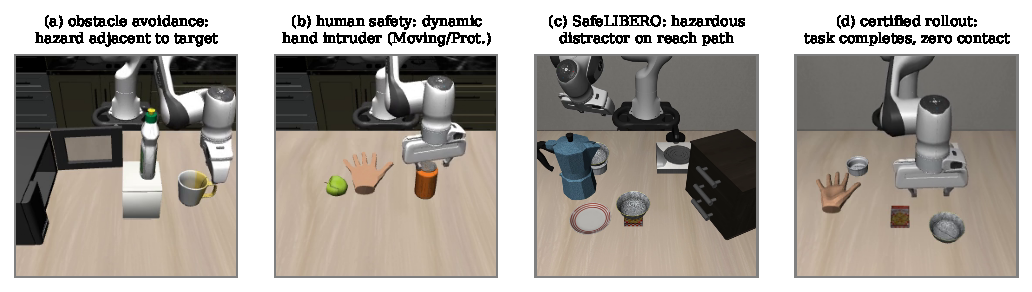
\includegraphics[width=0.98\textwidth]{fig_scenes.pdf}
\caption{Simulation testbeds. (a)~LIBERO-Safety obstacle avoidance: the elected guard (a spillable bottle) sits directly beside the task target. (b)~Human-safety suite: a hand enters the workspace mid-episode and is captured online by the \textsc{Moving}/\textsc{Protected} literals. (c)~SafeLIBERO: a hazardous distractor placed on the reach path. (d)~A certified rollout: the task completes with zero hazard contact under the checked prefix certificate.}
\label{fig:scenes}
\end{figure*}

\section{Experiments}
\label{sec:results}

\emph{Setup.} Frozen $\pi_{0.5}$~\cite{pi05} flow VLA; two benchmarks: SafeLIBERO~\cite{sota2607} (LIBERO tasks with a hazardous distractor near the reach path; collision $=$ $>$1\,mm ground-truth hazard displacement) and LIBERO-Safety~\cite{liberosafety} (named-object hazards, dynamic human-hand intruders, affordance and safety-reasoning suites; the benchmark's own contact-predicate violations). All comparisons are paired against self-run baselines under one protocol.

\subsection{SafeLIBERO: the symbolic rule matches ground truth}
\label{sec:e3}

\begin{figure*}[t]
\centering
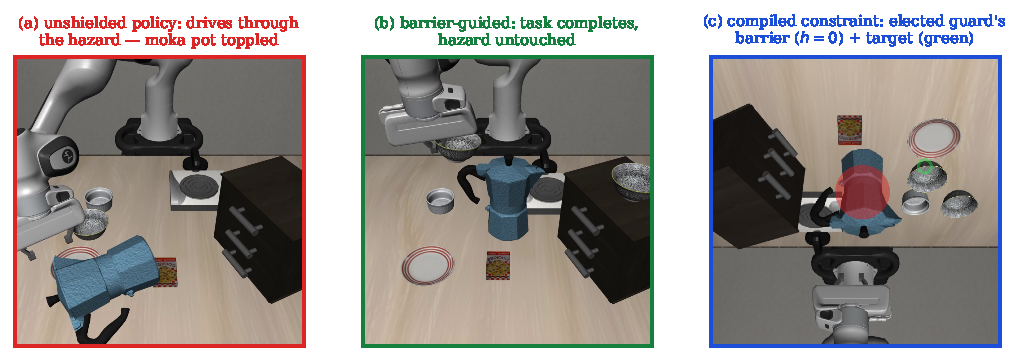
\includegraphics[width=0.95\textwidth]{fig_safelibero.pdf}
\caption{\textbf{SafeLIBERO, qualitatively.} (a)~An unshielded rollout: the policy drives through the hazardous distractor and topples the moka pot while reaching the bowl. (b)~A barrier-guided rollout on the same task family: the bowl is carried clear and the hazard is never touched. (c)~The compiled constraint, visualized: the FOL rule elects the moka pot ($\lnot\textsc{Mentioned}\wedge\textsc{NearestToPath}$; it is not named by the instruction and sits on the reach path), and its barrier's $h{=}0$ boundary (red) is projected into the camera view with the parsed target circled in green. The sphere-with-companions barrier plus per-step inflation is everything the enforcement layer sees --- symbols in, geometry out.}
\label{fig:safelibero}
\end{figure*}

\begin{table}[t]
\centering
\caption{Identification swap: enforcement fixed, \emph{only} the identity source varies. SafeLIBERO Spatial, $n{=}40$/arm/level, same seeds; TSR/CAR (\%). Paired McNemar GT vs.\ FOL: L1 TSR $p=0.55$; L1 CAR $p=0.50$; L2 TSR $p=0.18$; L2 CAR $p=1.0$.}
\label{tab:e3}
\begin{tabular}{lcc}
\toprule
Identity source & L1 TSR/CAR & L2 TSR/CAR \\
\midrule
Ground truth (simulator) & 55.0/27.5 & 77.5/40.0 \\
Symbolic + VLM priors & 60.0/27.5 & 77.5/37.5 \\
FOL rule, Eq.~\eqref{eq:fol} & 62.5/32.5 & 90.0/40.0 \\
\bottomrule
\end{tabular}
\end{table}

\begin{figure}[t]
\centering
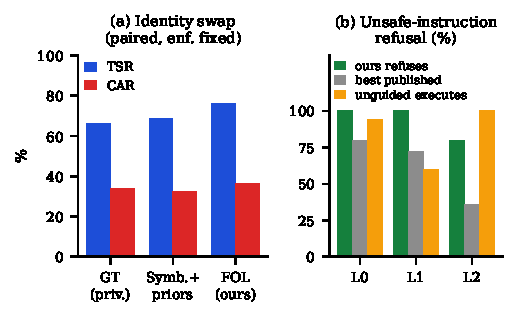
\includegraphics[width=0.99\columnwidth]{fig_results.pdf}
\caption{(a) Identification swap (Table~\ref{tab:e3}, Spatial L1/L2 mean): the ground-truth-free FOL rule matches privileged identity on both axes. (b)~Safety-reasoning suite: the symbolic instruction judge refuses unsafe instructions where the best published model partially complies --- and the unguided policy executes them.}
\label{fig:results}
\end{figure}

SafeLIBERO places a hazardous distractor near the reach path of standard LIBERO tasks (Fig.~\ref{fig:safelibero}); the unguided policy collides in up to 86--88\% of episodes. With the full stack, the ground-truth-free tier reaches 70.0\,TSR\,/\,46.5\,CAR on Spatial~L1 --- collision avoidance $2$--$3\times$ the unguided baseline's (14.0) at matched task success --- and dominates both a post-hoc shield and the reimplemented in-denoising SOTA on both axes in half the benchmark's cells. The identification-side evidence is the controlled experiment: Table~\ref{tab:e3} holds the enforcement stack fixed and swaps only the identity source. The ground-truth-free FOL rule is statistically indistinguishable from privileged simulator identity (all $p\ge0.18$), and every trend favors the rule (pooled discordant episodes 12:6 in its favor). The residual cost of removing privileged state is \emph{geometric} (localization error), not semantic. A deliberate-corruption study shows the failure direction: forcing the second-best identity pick costs collision avoidance (70$\to$25\%), not task success --- identification errors fail \emph{unsafe}, which is why the identification layer, not the barrier, is the reliability-critical component.

\subsection{VLM predicate grounding: same decisions, more competence}
\label{sec:grounding}

On 59 LIBERO-Safety scenes, replacing the rule's hand heuristics with VLM-answered \textsc{Referenced}/\textsc{Protected} predicates reproduces the \emph{identical} guard election on every scene (obstacle suite 12/13 top-1 and top-2 both; human suite 12/12 both), while resolving cases no string heuristic can: ``deliver it to me'' grounds the hand as \textsc{Protected}; a plate held by a hand is both \textsc{Referenced} and \textsc{Protected}. Offline on the same benchmark, the rule beats a flat VLM hazard-prior scorer (obstacle 12/13 vs.\ 9/11 top-1/top-2), because free-form semantic priors pull semantically-alarming \emph{names} (ketchup, tomato sauce) above the benchmark's designated obstacle --- geometry-plus-mention logic matches the safety-relevant entity.

\subsection{More neural authority fails unsafe}
\label{sec:negative}

Each escalation below was implemented, pre-registered, and killed by its own gate.

\textbf{Whole-scene VLM identification} (the field-default architecture: show the image, ask for the hazard) scores 18--64\% with API-strength models and 0--10\% with local models on scenes where the decomposed rule scores 100\%. The decomposition claim survives at every model scale we tested.

\textbf{VLM rule composition.} Letting a VLM \emph{compose} the identification rule from a groundable predicate library bounds the approach from above with oracle grounding: the entire compositional apparatus gains at most one scene and loses one to selection brittleness. With real VLM critics (two vendors), composition is strictly worse than the fixed rule on every suite (13/16 and 11/13 vs.\ 16/19 scenes), and the characteristic failure is an over-restrictive conjunction that fires on \emph{nothing}: 2 and 10 empty-rule scenes respectively, each leaving the true hazard unguarded. A safety component whose failure mode is silent unprotection is disqualified regardless of average accuracy.

\textbf{Scene-graph identification} exactly ties the flat scorer wherever hazards are objects (19/19 agreement) and collapses identically on the relational human suite --- where the fix is a 10-line \textsc{Protected} class rule, not structure.

\textbf{Safety prompting.} Instructing the policy to be careful moves task behavior but never collision avoidance across four testbeds --- the language channel of the VLA is behaviorally live yet safety-inert, ruling out the cheapest ``neural-only'' fix.

\subsection{System-level results on LIBERO-Safety}
\label{sec:ls}

\begin{table}[t]
\centering
\caption{Five-architecture board on LIBERO-Safety physical suites (TSR\,/\,violation\%; $n{=}150$ per suite, obst.-human $n{=}750$; macro = suite mean of TSR\,/\,viol.\,/\,safe-SR). All arms share one policy, protocol, and violation criterion; comparisons are against our self-run baseline at execution parity. \textbf{Bold}: best TSR per suite.}
\label{tab:board}
\small
\setlength{\tabcolsep}{3pt}
\begin{tabular}{lccccc}
\toprule
Arm & Obstacle & Human & Obst.-hum. & Afford. & Macro \\
\midrule
$\pi_{0.5}$ baseline & 74.0/4.0 & 84.0/0 & \textbf{69.3}/5.3 & \textbf{56.7}/0 & 71.0/2.3/70.0 \\
Post-hoc shield & 75.3/2.7 & 37.3/0 & 46.0/2.0 & 51.3/0 & 52.5/1.2/52.0 \\
SOTA reimpl. & 70.7/0.7 & 32.7/0 & 48.0/1.3 & 48.7/0 & 50.0/0.5/49.5 \\
Ours (GT) & \textbf{79.3}/4.7 & 78.7/0 & 63.2/1.9 & \textbf{58.7}/0 & 70.0/1.6/68.7 \\
Ours (no-GT) & 68.7/0.7 & \textbf{88.7}/0 & 58.9/1.7 & 56.0/0 & 68.1/0.6/67.9 \\
\bottomrule
\end{tabular}
\end{table}

Table~\ref{tab:board} places the full stack --- symbolic identification and routing, VLM predicate grounding, barrier-certified steering --- against the unshielded policy and two shield architectures. Both our arms beat both dedicated safety shields by $+15$--$20$ macro TSR at equal-or-lower violations: the shields pay their safety with task collapse on the human and affordance suites, where the symbolic routing (disengage on hazard--destination duality; property theory electing nothing on benign scenes) keeps ours task-capable. Against the \emph{unshielded} baseline, the GT arm beats it outright on obstacle avoidance and matches macro TSR within 1.0 at 30\% fewer violations; the ground-truth-free arm runs at a quarter of baseline's violation rate (0.6 vs.\ 2.3), beats it on human-safety (88.7 vs.\ 84.0), and holds macro safe-SR within 2.1 --- with the VLM-grounded property tables \emph{outscoring} the hand-token ablation on affordance (56.0 vs.\ 47.3): open-vocabulary grounding is both more general and more accurate than the hand lists it replaces. The residual no-GT deficit is localized to zero-slack scenes where centimeter-level localization error displaces the barrier into the work corridor --- a geometric tax, not a semantic one, consistent with Sec.~\ref{sec:e3}.

Separately, on the benchmark's safety-reasoning track the symbolic instruction judge refuses 100/100/80\% of unsafe instructions (levels L0/L1/L2) with zero violations, versus the best published model's 80/72/36\% --- while the unguided policy \emph{executes} the same unsafe instructions at 94/60/100\%. The policy hears language and complies; it does not judge. A learned consequence model as a task-progress tie-breaker among certified candidates matches the hand-tuned engagement gate within noise on the obstacle suite; by the certificate's mechanism independence, the identification findings above are insensitive to that enforcement-side choice.

\section{Discussion}
\label{sec:discussion}

\textbf{Why the division of labor works.} The predicates the rule consumes are local, verifiable, and cheap to audit: \textsc{Referenced} and \textsc{Protected} have single-object ground truth a human (or a test suite) can check, and errors surface as a wrong literal, not a wrong behavior. Scene-level judgment concentrates all failure into one uninspectable output; rule composition adds a synthesis step whose failure mode (empty conjunctions) is silent. The logic layer is where reliability properties --- fail-direction, monotonicity (semantics may add protection, never remove it), and routing transparency --- can be stated and enforced by construction.

\textbf{Limitations.} Benchmark cells are $n{=}40$--$50$ single-seed; the instruction judge's lexicon is in-domain (an upper bound pending held-out phrasings); rotation channels are uncertified; and the no-GT tier consumes the symbolic object \emph{name} list --- pixel-only naming currently costs identification and is future work. The rule itself is fixed: we claim no coverage beyond manipulation scenes with a nameable hazard set, and expect open-world deployment to require growing the \emph{predicate library} (the neural side) rather than the rule (the symbolic side) --- which is precisely the scaling direction this architecture makes cheap.

\section{Conclusion}
A three-literal first-order rule with VLM-grounded predicates identifies hazards as well as privileged ground truth; every escalation of neural authority we tested degrades it, unsafely. Embodied safety stacks should let the VLM ground symbols and the logic decide --- and certify enforcement by checking outputs, so the guarantee survives whatever neural machinery generates the motion.

\bibliographystyle{IEEEtran}
\begin{thebibliography}{20}

\bibitem{pi05} Physical Intelligence, ``$\pi_{0.5}$: A vision-language-action model with open-world generalization,'' arXiv:2504.16054, 2025.

\bibitem{liberosafety} Anonymous, ``LIBERO-Safety: Benchmarking safety-aware manipulation for vision-language-action models,'' arXiv:2606.23686, 2026.

\bibitem{sota2607} Anonymous, ``Neuro-symbolic safety guidance for vision-language-action models via constrained flow matching,'' arXiv:2607.01378, 2026.

\bibitem{aegis} Anonymous, ``AEGIS: A geometric safety shield for vision-language-action policies,'' arXiv:2512.11891, 2025.

\bibitem{safediffuser} W.~Xiao et al., ``SafeDiffuser: Safe planning with diffusion probabilistic models,'' arXiv:2306.00148, 2023.

\bibitem{cbf2602} Anonymous, ``Constricting barrier functions for certified diffusion policy safety,'' arXiv:2602.21429, 2026.

\bibitem{yourmodel} Anonymous, ``Your model already knows: Reading VLA attention for obstacle-aware control,'' arXiv:2606.09749, 2026.

\bibitem{brunke2025semantic} L.~Brunke et al., ``Semantically safe robot manipulation: From semantic scene understanding to motion safeguards,'' \emph{IEEE Robotics and Automation Letters}, 2025.

\bibitem{gdino} S.~Liu et al., ``Grounding DINO: Marrying DINO with grounded pre-training for open-set object detection,'' in \emph{ECCV}, 2024.

\bibitem{agrawal2017dcbf} A.~Agrawal and K.~Sreenath, ``Discrete control barrier functions for safety-critical control of discrete systems with application to bipedal robot navigation,'' in \emph{Robotics: Science and Systems (RSS)}, 2017.

\end{thebibliography}

\end{document}
